\documentclass[English]{style/ic-tese-v3}

\usepackage[latin1,utf8]{inputenc}

\usepackage
%  [pdfauthor={nome do autor},
%   pdftitle={titulo},
%   pdfkeywords={palavra-chave, palavra-chave},
%   pdfproducer={Latex with hyperref},
%   pdfcreator={pdflatex}]
{hyperref}
\usepackage{indentfirst}
\usepackage[T1]{fontenc}
\usepackage{titlesec}
\usepackage{subfig}
\titlespacing{\chapter}{0pt}{0pt}{0pt}

\titleformat{\chapter}%
  {\normalfont\bfseries\Huge}{\thechapter.}{10pt}{}

\titleformat{\chapter}{\normalfont\bfseries\huge}{\thechapter}{10pt}{\huge\bf\vspace{5mm}}
\usepackage{adjustbox}
\usepackage{amsmath}
\usepackage{multirow}
\usepackage{float}
\usepackage{pgfplotstable}
\usepackage{pgfplots}
\pgfplotsset{compat=1.13}
\usepackage{caption}
\captionsetup[table]{skip=5pt}

\begin{document}

% Escolha entre autor ou autora:
\documento{Research Project}

\autor{Erik de Godoy Perillo}
\titulo{Attention as a leverage for Deep Learning}
\orientadora{Prof.a. Dr.a. Esther Luna Colombini}

\paginasiniciais
\section*{Abstract}
Attention is fundamental for intelligent beings.
It is necessary for filtering the significant volumes of stimuli we constantly receive
and for applying the adequate mental resources to perform tasks.
Deep Learning is currently broadly applied to Artificial Intelligence.
The use of Attention in Deep Learning has been increasingly frequent,
resulting many times in better results.
In this context, this work proposes the study and elaboration of approaches to use Attention in Deep Learning
for more power and efficiency to solve problems in Artificial Intelligence.
We aim at obtaining techniques more generically applicable in broad problem classes
such as Computer Vision, Natural Language Processing, Differential Programming and others.
\fimdaspaginasiniciais


\chapter{Introduction}
We continually receive high volumes of multimodal stimuli from both external sources
-- such as visual, auditive signals -- and internal sources -- proprioception, memories et cetera.
It would be very inefficient or even impossible to process all the information with
the same intensity once a significant portion of it is irrelevant for
the task executed at the moment and considering that we have limited cognitive capacity.
When we read, our vision does not focus on all
words equally, but instead on a small subset of the text at a time.
When we are addressing a given subject (in a `'train of thought''), it tends to mediate the focus
in the memory search process, essentially retrieving memories that
are useful whereas many other irrelevant memories are not used.
It often happens that something conspicuous
-- such as a bird abruptly appearing in front of us or a sudden sound --
quickly draws our focus, `'stealing'' it from what was previously being focused.
The abilities to filter and select stimuli that are relevant for a task, to keep the focus for an
extended period and to adequately direct mental processes is fundamental to
human beings and other sophisticated forms of life.
We name this set of abilities `'Attention''~\cite{ref:esther-thesis}.

Attention can potentially play an essential role in Artificial Intelligence (AI).
The pursue of intelligent machines is an old effort in Computer Science~\cite{ref:turing} and is still very
relevant today due to the potential to radically benefit society.
Although there have been significant advancements in the field of AI, it is broadly accepted that
machines still cannot perform certain complex tasks nearly as efficiently as humans or some animals and
the path to achieving more intelligence is still unclear, with many different proposals~\cite{ref:mikolov}.
Part of the problem comes from the difficulty to properly define `'intelligence'' itself, but
surveys of the works on the subject~\cite{ref:aidef} suggest that a reasonably accepted
concept is the ability to perform elaborate tasks in complex and dynamic environments
in order to achieve a wide variety of goals.
From the narrow to the broader aspects of intelligence, the functionalities of Attention
are of great importance -- and it increases
as the level of intelligence considered increases~\cite{ref:helgason}.

A considerable amount of advancements in AI in recent years comes from
the popularization of Deep Learning (DL)~\cite{ref:dl}.
As we will discuss in the following sections, the technique mostly consists of
artificial neural networks architectured in a hierarchical manner.
DL showed to be effective in a variety of tasks in computer vision~\cite{ref:imagenet}\cite{ref:segmentation},
audio processing~\cite{ref:wavenet} and Natural Language
Processing (NLP)~\cite{ref:att-all-you-need}, mainly due to its ability
to learn what features should be extracted (rather than relying on hand-crafted features).
Along with the transposition from classic models to DL
approaches, an increasingly high number of works on the field
have been using concepts related to Attention in combination with DL to achieve better results.
One example is image captioning (figure \ref{fig:description}) where the task
consists of giving a natural language description of a given image.
The work presented in ~\cite{ref:img-captioning} shows that the task benefits from
sequentially focusing on different parts of the image in a sequence,
through the use of an attentional component in the model.
Other examples -- which will be discussed in-depth in following sections -- include linguistic
translation~\cite{ref:translation}, audio recognition~\cite{ref:audio} and neural computation~\cite{ref:ntm}.
These are evidence that concepts of Attention have indeed been useful for the field.

\begin{figure}
\begin{center}
	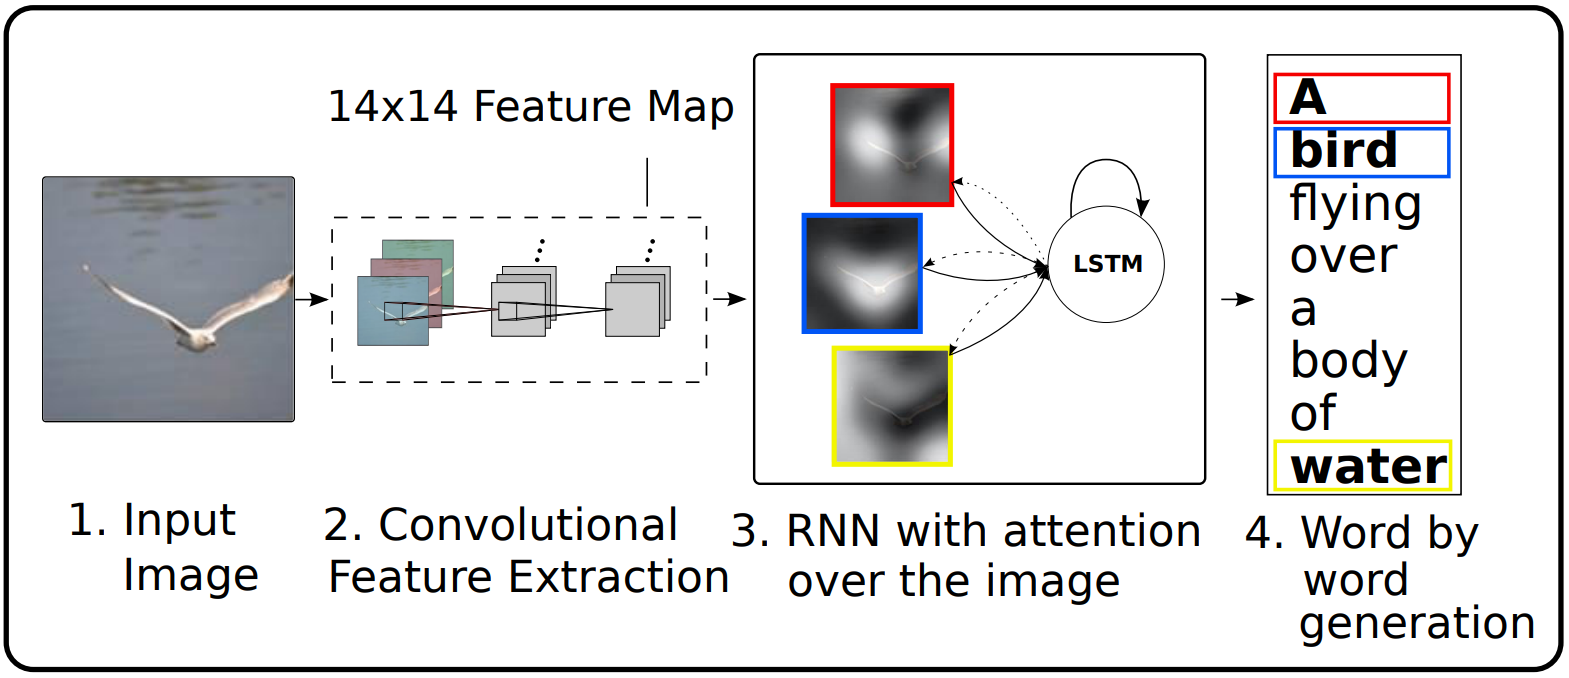
\includegraphics[width=1.0\linewidth]{./img/img_captioning.png}
\caption{
    Diagram of natural language image description using Attention
    (from \cite{ref:img-captioning}).
}
\label{fig:description}
\end{center}
\end{figure}

\section{Objectives}
In spite of the recent adoption of Attention by a variety of Deep Learning models
and the significant improvements it has shown, it is conjectured that there are still many other tasks
that are still not very well explored.
Current works also tend to focus more on the filtering functionality of Attention,
but there are other aspects
-- such as the allocation of mental resources in the course of time -- that can be of potential benefit
(we further discuss the taxonomy of Attention in following sections).
Furthermore, we note that Attention models currently being used
are very specific to each problem in question.
Some works propose a higher level of generalization~\cite{ref:recurr-models},
but we believe it is possible to go further.
Therefore, the specific objectives of this work are:
\begin{itemize}
    \item To perform an extensive literature review on the use of Attention
        in modern Deep Learning techniques;
    \item To identify specific problems in different classes
        (robotics, vision, NLP, differential programming) with
        improvement potential by the use of Attention;
    \item To identify more theoretical aspects of Attention itself and their applicabilities to Deep Learning;
    \item To propose and implement one or more solutions based on the findings of the work in order to
        validate the ideas and evaluate them in an application.
    \item To study the viability of generalization of Attention
        to broader areas in AI other than Deep Learning.
\end{itemize}

\chapter{Background}
\section{Attention}
The interest in the concept of attention exists since a long time ago.
Throughout the years, attention has been studied
from various perspectives (c) such as philosophy, psychology, and neurology.
Thus, there are multiple definitions of the concept.
In broad terms, we can define attention as
\emph{the act of guiding the processing of information
according to a critical evaluation method that is specific to a particular task at a given time}.
In the next items, we discuss some concepts related to attention.

\subsection{Functionalities of attention}
Attention can be manifested in different manners depending on the goal (c).
The most common is the act of selecting a set of stimuli over others
(selective attention), such as looking at only a portion of an image.
Another component is the act of guiding how one's focus moves over time
(oriented attention), such as the act of looking at the words in
a sequential manner when reading.
Keeping the focus on a specific semantic element is important in some tasks
and is known as sustained attention.

\subsection{Bottom-up and Top-down attention}
Focus may emerge in two fundamentally different manners (c).
In bottom-up attention, the act of focusing is involuntarily
started and guided by (usually) external and conspicuous stimuli,
such as a shattering glass that tends to
make us immediately turn our heads towards where the noise came from.
Another example is visual saliency (figure \ref{fig:saliency}):
a glowing red ball suddenly appearing in
your field of vision will probably grab your focus.
In top-down attention, focus is voluntarily guided by cognition and goals.
If we are talking to someone in a crowded party, for example,
we focus on what the specific person is saying
-- ignoring other people's words -- in order to maintain the conversation.

\begin{figure}
\begin{center}
		\begin{tabular} {cc}
		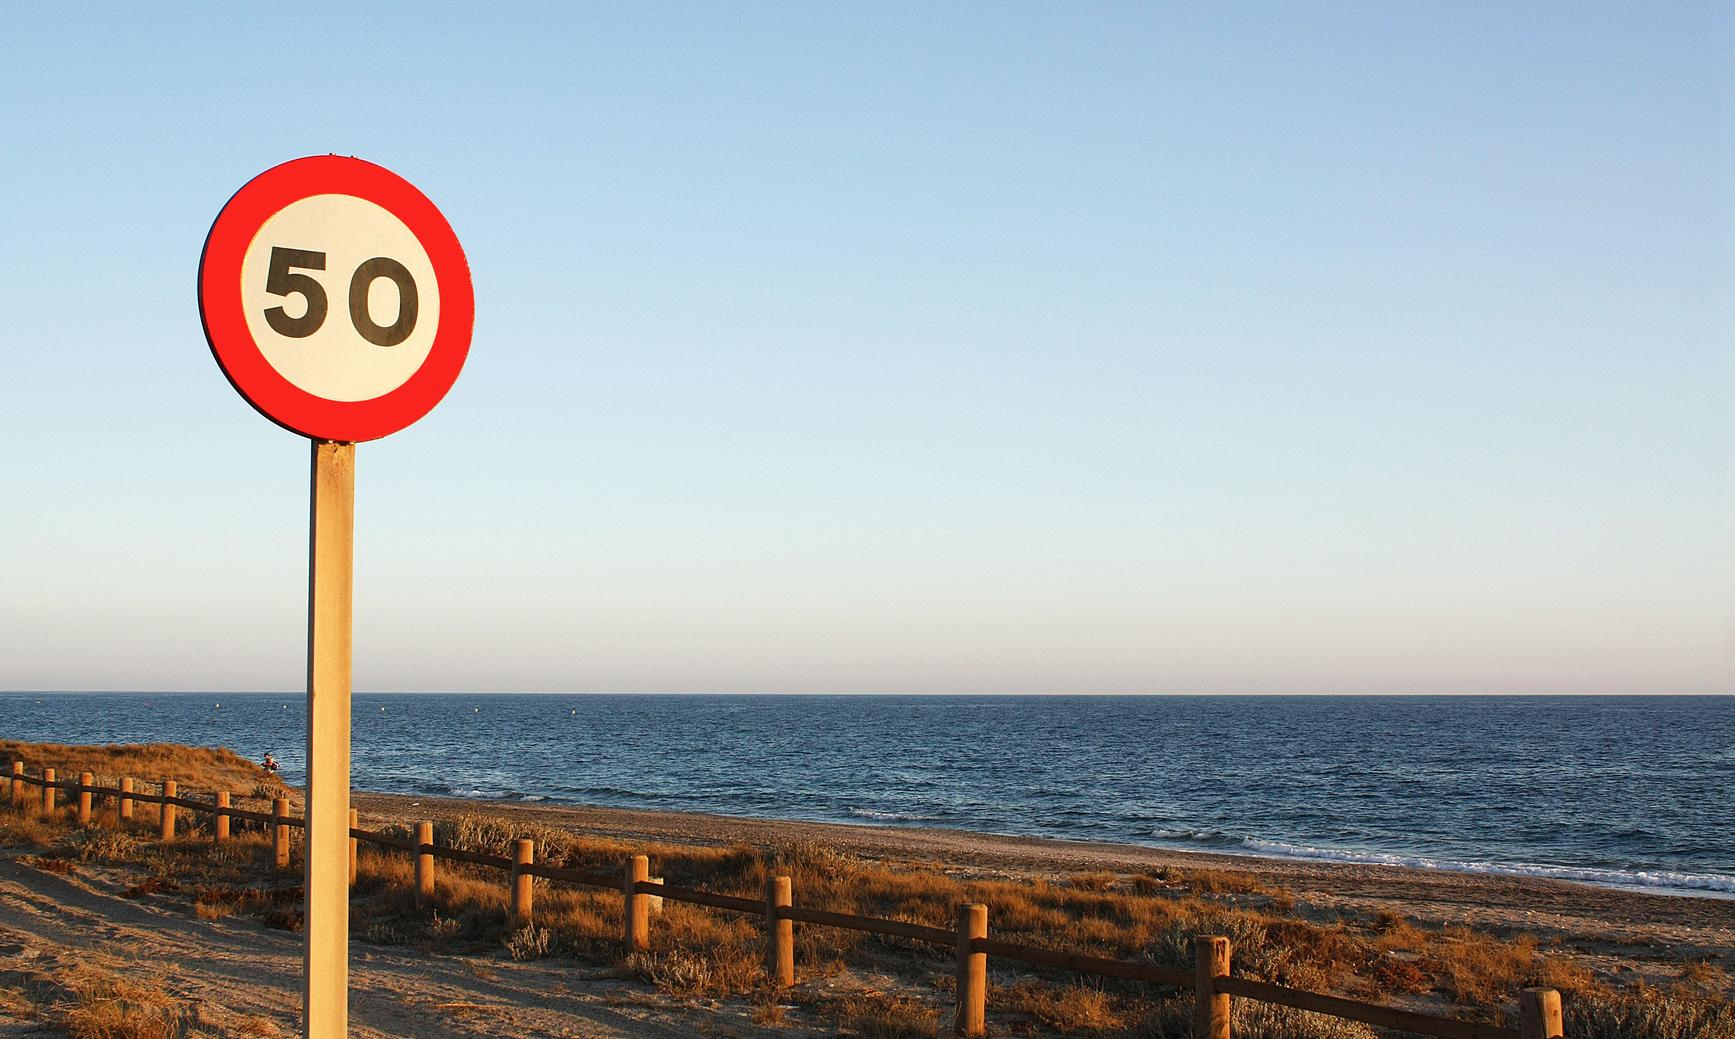
\includegraphics[width=0.45\linewidth]{./img/traffic_sign_s.jpg} &
		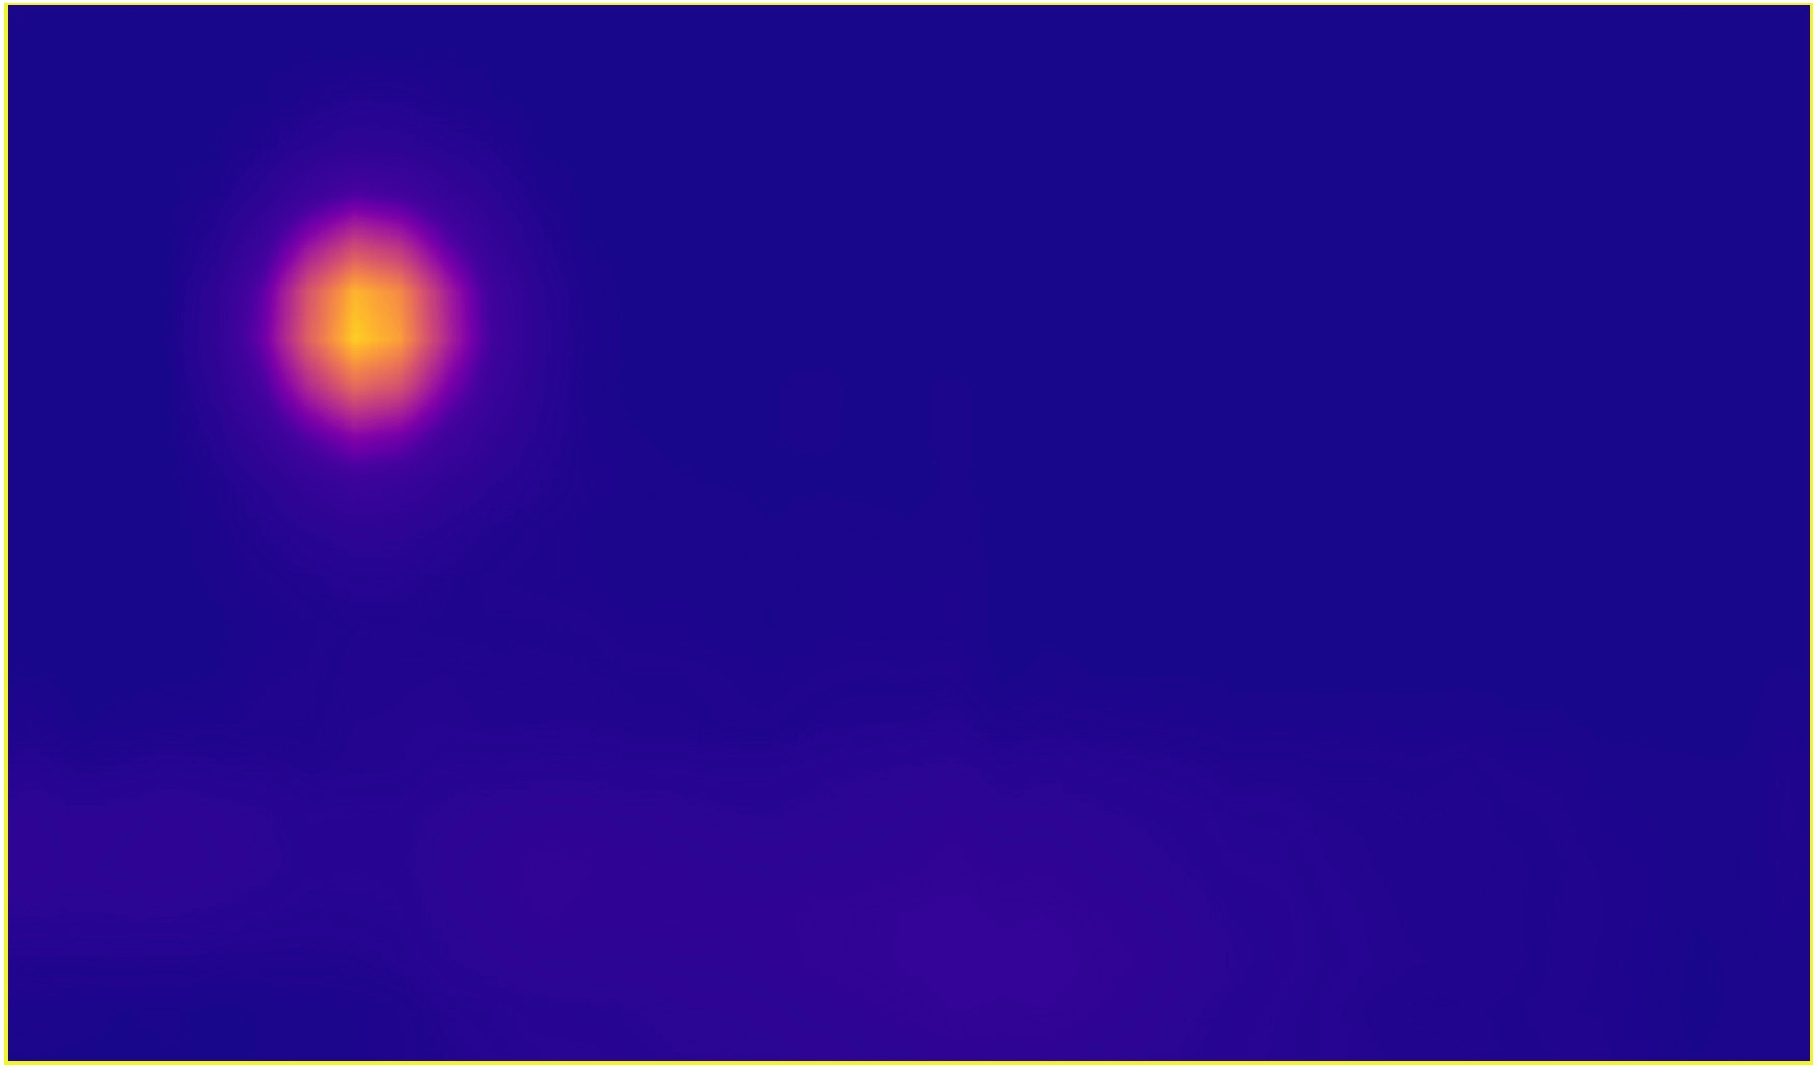
\includegraphics[width=0.45\linewidth]{./img/traffic_sign_m.jpg}\\
        (a) & (b)
		\end{tabular}
\caption{Exemple of visual saliency.
    b) is the saliency map where higher intensity pixels represent
    regions that are more salient to humans than original image a).}
\label{fig:saliency}
\end{center}
\end{figure}

\subsection{Soft and Hard attention}
In recent years, there has been an useful distinction between
soft and hard attention (c).
Soft attention regards defining a continuous distribution of importance
across all elements of information for some task.
In the example of visual saliency, one can determine a saliency map $M$
to a given image $I$ where each pixel will have a value in $[0, 1]$
regarding its saliency.
Hard attention regards determining a discrete subset of
important information elements.
Using again the problem of visual saliency as an example,
one might want to determine a specific location $(i, j)$ of the image
to be used as center of a small patch of the image that is the most
relevant to be further processed.

\section{Deep Learning}
Deep Learning (DL) is a trend in modern AI (c).
Although DL started being broadly adopted around x years ago,
some of its concepts date to much earlier than that (c):
foundations of artificial neural networks were already discussed
in the 1950s, backpropagation was introduced in the 1970s
and many other key concepts that are popular mostly in the last decade or less
were introduced more than 30 years ago.
Many fields of AI witnessed a major shift in paradigm
in the last years: models applying DL concepts now achieve state-of-the-art
results in different problems regarding computer vision (c)(c)(c),
audio processing (c), NLP (c), neural computation (c) among others.
DL used used both in supervised and unsupervised learning (c).

One of the key concepts of DL is that of hierarchy of features (c):
A deep sequence of layers apply non-linear transformations to the data
in such a way that many models learn to extract features of hierarchical
levels of abstraction.
For this reason, DL is also regarded as Representation Learning.
This characteristic enables such models to learn latent structure
in intrinsically unstructured data such as images, text and audio signals.
Another advantage is that of transfer learning: models that are
primarily trained for a given task can be used and adapted for another
task while using at least part of the representations learned.
We discuss some concepts related to DL in following items.

\subsection{Artificial Neural Networks (ANNs)}
ANNs are usually adopted to prediction
learning problems by means of learning a non-linear function aproximation.
The ideas used in ANNs date to more than 50 years ago (c) and many of them
are inspired from observed mechanisms of the human brain (x).
Most of DL models are a variation of one of the families of ANNs
that will be briefly discussed here.

One of the most basic examples is that of Multi Layer Perceprons (MLPs).
The main caracteristic of this model is the use of hidden layers
and neurons are a linear combination of previous layers followed by
a non-linear activation.
Each layer $l_k$ (with $n$ neurons) is connected to the previous layers
$l_{k-1}$ (with $m$ neurons) and the neuron $l_k^i$, $1 \le i \le n$
is given value:
$$l_k^i = h\left(\sum_{j=1}^{m} l_{k-1}^jw_k^j + b_k^j\right)$$
%Where $h(x): \mathbb{R} \mapsto \mathbb{R}$ is a non-linear activation funcion.
Commonly commonly used functions are the sigmoid hyperbolic tangent
and the Rectified Linear Unit (ReLU):
$$f(x) = \begin{cases}
    0, & x < 0 \\
    x, & x \ge 0 \\
        \end{cases}
$$
ReLU is a currently broadly adopted due to its high efficiency
and training speed (c).

\begin{figure}
\begin{center}
    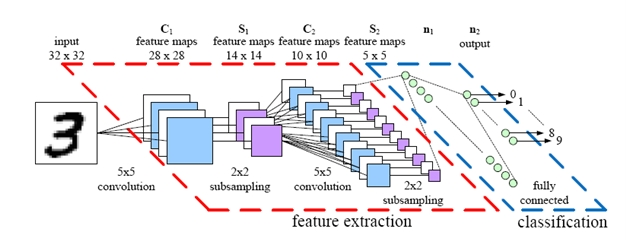
\includegraphics[width=1.0\linewidth]{./img/cnn.png}
\caption{
    Diagram of a convolutional neural network.
    Learned filters extract features in an increasingly hierarchical manner.
}
\label{fig:cnn}
\end{center}
\end{figure}

Convolutional Neural Networks (CNNs) are widely used
in computer vision
tasks such as image classification, localization and semantic segmentation.
CNNs use the fact that images tend to have correlated pixels and use
convolution filters in an hierarchical manner (figure \ref{fig:cnn})
to learn features in increasing abstraction.
For a certain layer, the $i$-th feature map $m_i$ is,
given filter weights $W_i$, bias $b_i$ and nonlinearity function $h(x)$,
obtained as:
$$m_i = h\left(W_i * x + b_i\right)$$
with $*$ as the convolution operation.

Recurrent Neural Networks (RNNs) are characterized by a recursive architecture
that uses the input of the current step and the output of the previous
step to compute the predictions.
The hidden state $h_t$ at time step $t$, given input $x_t$, weight matrix $W$,
previous state $h_{t-1}$, hidden-state-to-hidden-state matrix $U$ and
non-linearity $f(x)$ is given by:
$$h_t = f\left(Wx_t + Uh_{t-1}\right)$$
These architectures are widely used in NLP tasks (c) such as
machine translation (c).
Some variations over the original basic architecture such as
LSTMs (c) are also broadly adopted.

\subsection{Learning process}
The act of learning the appropriate weights of a given model
is usually obtained by the minimization of a differentiable loss function
that is based on the cost function $L(y, \hat{y})$ that characterizes the error
between the true value $y$ and the predicted value $\hat{y}$.
Backpropagation (c) plays an important role in DL because it's used
to adjust the weights $\theta$ of models that have a
differentiable cost function.
A typical training process is composed of a forward-propagation
step which computes the predictions over a set of input samples
and a backpropagation step which computes the loss function
and adjusts the weights of the model.
In DL, acommon such adjustment methods include Stochastic Gradient Descent (SGD)
which, for a given minibatch, adjusts weights according to:
$$\theta_{i+1} = \theta_i - \alpha\frac{\partial{J}}{\partial{\theta}}$$
where $\alpha$ is the learning rate.

\let\clearpage\relax

\chapter{Related Work}
TODO: detailed examples on DL + attention.
maybe cite our previous work here?
%In vision, we can cite problems such as visual saliency
%(figure \ref{fig:saliency}): In a given image, which region should be
%first focused on? Older computacional models generally extracted
%hand-crafted features regarding color, luminance and image
%statistics~\cite{ref:judd}.
%A significant boost in performance~\cite{ref:mit300-bm} was achieved
%with the adoption of Deep Learning models with arquitechture components
%specifically designed for the context of saliency detection ~\cite{ref:deepfix}
%~\cite{ref:salicon}~\cite{ref:mlnet}.
%In previous work~\cite{ref:erik-esther}, which is result from a Undergraduate
%Research project conducted by the author
%-- and received `'best undergraduate research project'' award from
%the institute of computing at Unicamp in 2017 --
%we developed a fully convolutional neural network that emcompasses
%arquitechture and data processing specifically design for the saliency
%detection task.
%While having similar performance to that of top models
%(in the MIT Saliency Benchmark) at the time,
%the model was composed of significantly less parameters than other models.

\let\clearpage\relax

\chapter{Methodology}
TODO:
\begin{itemize}
    \item description of stages: lit review,
        search for problems, generalization, application
\end{itemize}

\section{Schedule}
TODO: the schedule.

\renewcommand\bibname{References\vspace*{10mm}}

\begingroup
\let\clearpage\relax
\bibliographystyle{plain}
\bibliography{proposal.bib}
%\printbibliography
\endgroup

\end{document}
